\documentclass[11pt,a4paper]{article}

% =============================================================================
% PACKAGE IMPORTS
% =============================================================================
\usepackage[utf8]{inputenc}
\usepackage[T1]{fontenc}
\usepackage{times}
\renewcommand{\sfdefault}{lmss}
\renewcommand{\ttdefault}{lmtt}
\usepackage{microtype}
\usepackage{geometry}
\geometry{margin=1in}

\usepackage{amsmath,amssymb,amsfonts,mathtools}
\usepackage{graphicx}
\graphicspath{{output/}{./}}
\usepackage{booktabs}
\usepackage{multirow}
\usepackage{tabularx}
\usepackage{array}
\usepackage{xcolor}
\usepackage{hyperref}
\usepackage{enumitem}
% \usepackage{algorithm}
% \usepackage{algorithmic}
\usepackage{cite}
\usepackage{caption}
\usepackage{subcaption}
\usepackage{tikz}
\usetikzlibrary{shapes.geometric, arrows.meta, positioning, calc, fit, backgrounds}

% Hyperlink configuration
\hypersetup{
    colorlinks=true,
    linkcolor=navyblue,
    citecolor=darkgreen,
    urlcolor=navyblue
}

% Custom Colors
\definecolor{navyblue}{RGB}{0,32,96}
\definecolor{darkgreen}{RGB}{0,100,0}
\definecolor{crimsonred}{RGB}{160,0,0}
\definecolor{lightgray}{gray}{0.95}
\definecolor{softblue}{RGB}{226,240,255}
\definecolor{softgreen}{RGB}{224,245,230}
\definecolor{softorange}{RGB}{255,239,213}
\definecolor{softpurple}{RGB}{238,226,255}
\definecolor{softred}{RGB}{255,226,226}
\definecolor{borderblue}{RGB}{40,90,160}
\definecolor{bordergreen}{RGB}{30,130,60}
\definecolor{borderorange}{RGB}{190,100,20}
\definecolor{borderpurple}{RGB}{110,50,160}
\definecolor{borderred}{RGB}{170,40,40}

% =============================================================================
% TITLE & AUTHOR METADATA
% =============================================================================
\title{\textbf{\Large Self-Distillation with Frequency-Adaptive 2D Rotary Position Embeddings and Spatial-Semantic Sparse Attention for Vision Transformers}}

\author{
  \textbf{Pham Cung Le Nhan Vu}, \textbf{Nguyen Hoang Khang}, and \textbf{Nguyen Hoai Nam}\thanks{Faculty of Data Science, VNUHCM -- University of Science. Contact email: \texttt{25C01014@pos.hcmus.edu.vn}} \\[0.3em]
  Faculty of Data Science \\
  VNUHCM -- University of Science, Ho Chi Minh City, Vietnam
}

\date{\today}

\begin{document}
\maketitle

% =============================================================================
% ABSTRACT
% =============================================================================
\begin{abstract}
Self-supervised knowledge distillation without labels, notably pioneered by DINOv1, enables Vision Transformers (ViTs) to learn semantic representations exhibiting emergent scene segmentation and clustering capabilities. However, standard ViTs in self-supervised pipelines rely predominantly on learnable absolute positional embeddings (APEs) and dense multi-head self-attention. This classical formulation suffers from two fundamental limitations: (1) poor geometric generalization when processing multi-scale image crops due to rigid bicubic interpolation artifacts, and (2) quadratic computational complexity paired with diffuse attention dispersion, where uninformative background clutter (e.g., sky, ground) pollutes the central \texttt{[CLS]} representation. In this work, we propose a synergized architectural enhancement for self-supervised Vision Transformers comprising: (i) \textbf{Frequency-Adaptive 2D Rotary Position Embedding (2D RoPE)}, which decomposes spatial coordinate tokens along frequency spectra to balance local high-frequency boundary details with scale-invariant low-frequency global topology, and (ii) \textbf{Spatial-Semantic Sparse Attention}, which unifies local spatial window connectivity ($K_{\text{local}} \times K_{\text{local}}$), dynamic global semantic Top-$K$ routing, and bidirectional \texttt{[CLS]} token dispatch while strictly preserving standard Softmax probability normalization. We evaluate our approach in a modular PyTorch framework by pretraining without labels on \textbf{ImageNet-100} for \textbf{190 epochs} on an \textbf{NVIDIA H100 GPU}, and directly evaluating the frozen pretrained model on the \textbf{CIFAR-10} benchmark. On CIFAR-10, our model outperforms the baseline across all evaluation protocols, achieving \textbf{75.97\%} $k$-NN ($k=10$) Top-1 accuracy (+1.56\% over 74.41\%), \textbf{75.31\%} $k$-NN ($k=20$) Top-1 accuracy (+0.97\% over 74.34\%), \textbf{82.60\%} 30-epoch Linear Probing Top-1 accuracy (+2.14\% over 80.46\%), and \textbf{83.87\%} 100-epoch Linear Probing Top-1 accuracy (+2.57\% over 81.30\%). Remarkably, during 30-epoch linear probing, our method reaches \textbf{79.86\%} accuracy by epoch 10 compared to \textbf{73.76\%} for the baseline (+6.10\% convergence acceleration), with \textbf{zero parameter overhead} (exactly 21.67M backbone parameters) and identical theoretical FLOPs (9.20 GFLOPs). Qualitative attention visualizations demonstrate that our model produces sharply delineated object boundaries and effectively suppresses background noise.
\end{abstract}

\textbf{Keywords:} Self-Supervised Learning, Knowledge Distillation, DINOv1, Vision Transformer, Rotary Position Embedding (RoPE), Sparse Attention, Representation Learning.

% =============================================================================
% 1. INTRODUCTION
% =============================================================================
\section{Introduction}
\label{sec:intro}

Self-Supervised Learning (SSL) has reshaped modern representation learning across computer vision and natural language processing. In visual domains, self-distillation methods—particularly DINO (Distillation with no labels) \cite{caron2021emerging}—have demonstrated that Vision Transformers (ViTs) \cite{dosovitskiy2020image} trained without human annotations naturally acquire explicit scene semantics, object boundaries, and feature linear separability superior to supervised baselines.

Despite these empirical successes, canonical ViT architectures employed in DINOv1 retain architectural vestiges from standard sequence models that are suboptimal for visual data:
\begin{enumerate}[leftmargin=*]
    \item \textbf{Geometric Brittleness of Absolute Positional Embeddings:} Standard ViTs add learnable 1D or 2D Absolute Positional Embeddings (APEs) to image patch tokens prior to Transformer blocks. In self-supervised multi-crop training \cite{caron2020swav, caron2021emerging}, networks alternate between global crops ($224 \times 224$, $14 \times 14$ patches) and local crops ($96 \times 96$, $6 \times 6$ patches). Resizing static positional vectors via bicubic interpolation degrades relative spatial orientation, distorts high-frequency phase information, and ignores translation equivariance.
    \item \textbf{Attention Dilution in Dense Softmax Attention:} Dense Multi-Head Self-Attention scales quadratically $\mathcal{O}(N^2)$ with the patch sequence length $N$. More critically, fully dense attention allows semantic tokens to disperse attention mass indiscriminately over extensive background regions (such as cloudy skies or uniform pastures). This leads to representational pollution of the \texttt{[CLS]} token, hindering downstream classification and fine-grained boundary segmentation.
    \item \textbf{High Compute Overhead in Self-Supervised Training:} State-of-the-art SSL pipelines frequently require massive GPU clusters (e.g., 8 to 64 V100/A100 GPUs), creating substantial barriers for individual researchers and academic laboratories constrained by consumer hardware (e.g., 8GB VRAM).
\end{enumerate}

To address these challenges, we introduce an enhanced, resource-efficient self-supervised Vision Transformer architecture integrated into DINOv1. Our primary contributions are summarized as follows:
\begin{itemize}[leftmargin=*]
    \item \textbf{Frequency-Adaptive 2D Rotary Position Embedding (2D RoPE):} We extend Rotary Position Embeddings \cite{su2024roformer} to continuous two-dimensional visual grids with frequency-aware coordinate adaptation. High-frequency dimensions capture fine-grained pixel boundaries using raw coordinates, while low-frequency bands generalize to varying resolutions via normalized coordinates.
    \item \textbf{Spatial-Semantic Sparse Softmax Attention:} We design a composite sparse attention mechanism combining a local 2D Chebyshev spatial window, a dynamic global semantic Top-$K$ candidate selection, and bidirectional \texttt{[CLS]} routing. Additionally, we provide a multi-scale 2D sliding-window variant (\texttt{MultiScale2DWindowAttention}) grouping heads across $3\times 3$, $5\times 5$, $7\times 7$, and full global receptive fields. Both designs retain exact Softmax properties without probability truncation.
    \item \textbf{Modular Registry and Declarative Configuration Builder:} We implement a decoupled, clean PyTorch architecture featuring a dynamic component registry (\texttt{MODULES}, \texttt{BACKBONES}, \texttt{HEADS}, \texttt{LOSSES}, \texttt{OPTIMIZERS}, \texttt{TRANSFORMS}) allowing flexible network and training pipeline instantiation via declarative YAML configurations.
    \item \textbf{Empirical Validation via ImageNet-100 Pretraining and CIFAR-10 Evaluation:} Pretrained without labels on \textbf{ImageNet-100} for \textbf{190 epochs} on an \textbf{NVIDIA H100 GPU} and directly evaluated on \textbf{CIFAR-10}, our ViT-Small/16 variant achieves \textbf{75.97\%} $k$-NN ($k=10$) Top-1 accuracy (+1.56\%), \textbf{75.31\%} $k$-NN ($k=20$) Top-1 accuracy (+0.97\%), and up to \textbf{83.87\%} Linear Probing Top-1 accuracy (+2.57\% over 81.30\%), demonstrating +6.10\% faster convergence at early probe epochs while maintaining zero parameter overhead.
\end{itemize}

% =============================================================================
% 2. RELATED WORK
% =============================================================================
\section{Related Work}
\label{sec:related}

\subsection{Self-Supervised Visual Representation Learning}
Self-supervised visual learning paradigms have evolved from contrastive methods like MoCo \cite{he2020momentum, chen2021mocov3} and SimCLR to non-contrastive knowledge distillation frameworks like BYOL \cite{grill2020byol}, SwAV \cite{caron2020swav}, and DINO \cite{caron2021emerging}. DINO interprets self-supervised learning as knowledge distillation with no labels: a student network is trained to predict the output distribution of a dynamically momentum-updated teacher network. By combining multi-crop data augmentation with centering and sharpening operations on the teacher's probability distribution, DINO avoids trivial representation collapse without negative sample pairs. DINOv2 \cite{oquab2023dinov2} scaled this approach to billion-parameter datasets with register tokens \cite{darcet2024vision}. In contrast, our focus is optimizing architectural inductive biases and positional geometry under constrained compute budgets.

\subsection{Positional Encodings in Vision Transformers}
The canonical Vision Transformer \cite{dosovitskiy2020image} maps non-overlapping image patches to vectors and adds 1D learnable absolute positional embeddings. While functional for fixed-size classification, APE lacks relative translation invariance. Relative Positional Encodings (RPE) introduce distance biases directly into the attention logits. Rotary Position Embedding (RoPE) \cite{su2024roformer} was developed for autoregressive language modeling, encoding relative token distances through complex vector rotations. Recent vision adaptations extend RoPE to 2D image coordinates; however, existing methods apply uniform scaling across all channels, overlooking the disparate multi-scale demands of high-frequency local textures versus low-frequency global layouts.

\subsection{Sparse and Efficient Attention}
Dense multi-head attention suffers from $\mathcal{O}(N^2)$ time and memory scaling. Sparse Transformers \cite{child2019generating}, Longformer \cite{beltagy2020longformer}, and BigBird \cite{zaheer2020bigbird} demonstrated that sparse connectivity graphs combining local sliding windows and global routing achieve competitive representational power in long text sequences. Swin Transformer \cite{liu2021swin} pioneered shifted local windows for vision backbones. In our framework, we specifically tailor sparse connectivity for self-distillation: we blend local spatial proximity with semantic Top-$K$ content routing and full \texttt{[CLS]} token routing, preserving exact Softmax normalization and zero parameter overhead.

% =============================================================================
% 3. METHODOLOGY
% =============================================================================
\section{Methodology}
\label{sec:method}

% -----------------------------------------------------------------------------
% FIGURE 1: OVERALL SELF-DISTILLATION PIPELINE (LEFT-TO-RIGHT CLEAN LAYOUT)
% -----------------------------------------------------------------------------
\begin{figure*}[t!]
\centering
\resizebox{\textwidth}{!}{%
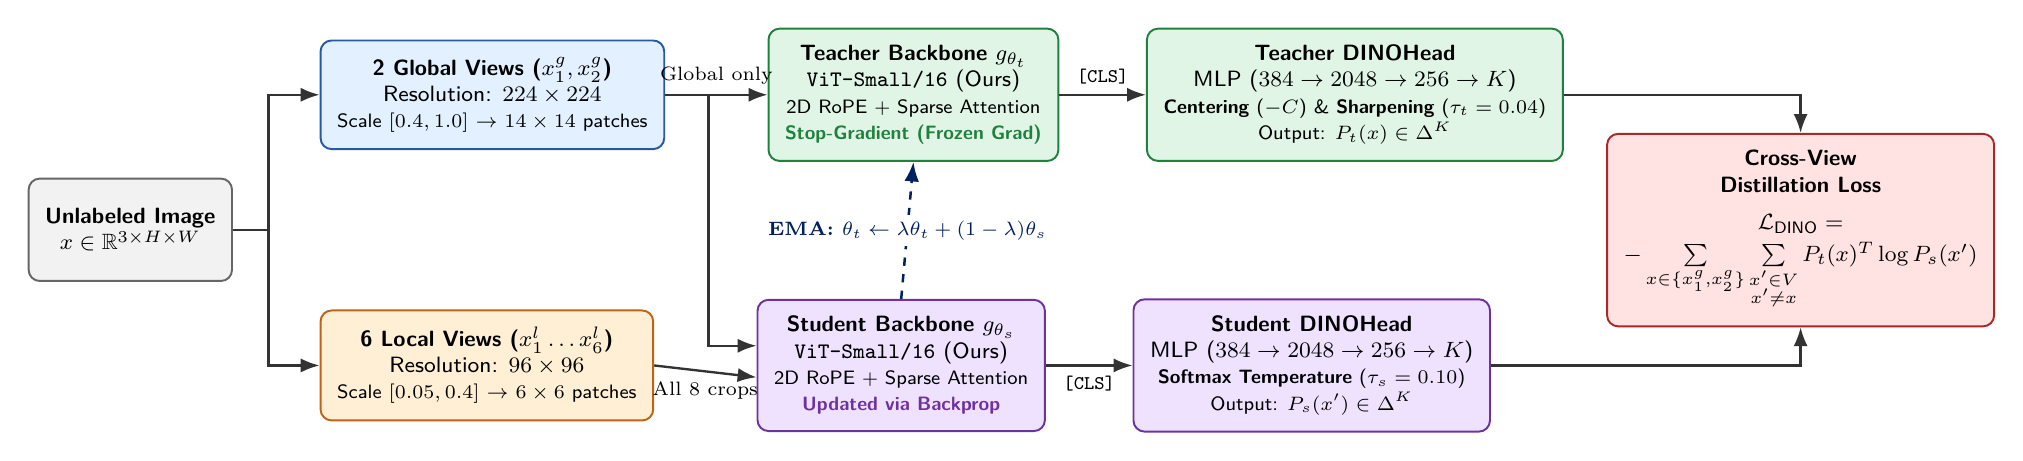
\begin{tikzpicture}[
    font=\sffamily\footnotesize,
    >=Latex,
    box/.style={draw=black!70, rounded corners=4pt, align=center, inner sep=6pt, line width=0.7pt},
    bluebox/.style={box, fill=softblue, draw=borderblue},
    greenbox/.style={box, fill=softgreen, draw=bordergreen},
    orangebox/.style={box, fill=softorange, draw=borderorange},
    purplebox/.style={box, fill=softpurple, draw=borderpurple},
    redbox/.style={box, fill=softred, draw=borderred},
    graybox/.style={box, fill=lightgray, draw=black!60},
    arrow/.style={->, line width=0.85pt, draw=black!80},
    emaarrow/.style={->, dashed, line width=0.9pt, draw=navyblue}
]

% 1. Input Image
\node[graybox, minimum width=2.3cm, minimum height=1.3cm] (input) {
    \textbf{Unlabeled Image}\\$x \in \mathbb{R}^{3\times H \times W}$
};

% 2. Multi-Crop Views (Top: Global, Bottom: Local)
\node[bluebox, minimum width=3.1cm, minimum height=1.2cm, above right=0.35cm and 1.1cm of input] (global_crops) {
    \textbf{2 Global Views ($x_1^g, x_2^g$)}\\
    Resolution: $224 \times 224$\\
    {\scriptsize Scale $[0.4, 1.0]$ $\rightarrow$ $14\times 14$ patches}
};

\node[orangebox, minimum width=3.1cm, minimum height=1.2cm, below right=0.35cm and 1.1cm of input] (local_crops) {
    \textbf{6 Local Views ($x_1^l \dots x_6^l$)}\\
    Resolution: $96 \times 96$\\
    {\scriptsize Scale $[0.05, 0.4]$ $\rightarrow$ $6\times 6$ patches}
};

% 3. Teacher and Student Backbones
\node[greenbox, minimum width=3.5cm, minimum height=1.35cm, right=1.3cm of global_crops] (teacher_net) {
    \textbf{Teacher Backbone $g_{\theta_t}$}\\
    \texttt{ViT-Small/16} (Ours)\\
    {\scriptsize 2D RoPE + Sparse Attention}\\
    {\scriptsize \textcolor{bordergreen}{\textbf{Stop-Gradient (Frozen Grad)}}}
};

\node[purplebox, minimum width=3.5cm, minimum height=1.35cm, right=1.3cm of local_crops] (student_net) {
    \textbf{Student Backbone $g_{\theta_s}$}\\
    \texttt{ViT-Small/16} (Ours)\\
    {\scriptsize 2D RoPE + Sparse Attention}\\
    {\scriptsize \textcolor{borderpurple}{\textbf{Updated via Backprop}}}
};

% 4. DINO Heads & Distributions
\node[greenbox, minimum width=3.2cm, minimum height=1.35cm, right=1.1cm of teacher_net] (teacher_head) {
    \textbf{Teacher DINOHead}\\
    MLP ($384 \to 2048 \to 256 \to K$)\\
    {\scriptsize \textbf{Centering} ($-C$) \& \textbf{Sharpening} ($\tau_t=0.04$)}\\
    {\scriptsize Output: $P_t(x) \in \Delta^K$}
};

\node[purplebox, minimum width=3.2cm, minimum height=1.35cm, right=1.1cm of student_net] (student_head) {
    \textbf{Student DINOHead}\\
    MLP ($384 \to 2048 \to 256 \to K$)\\
    {\scriptsize \textbf{Softmax Temperature} ($\tau_s=0.10$)}\\
    {\scriptsize Output: $P_s(x') \in \Delta^K$}
};

% 5. Cross-View Distillation Loss
\coordinate (mid_heads) at ($(teacher_head.east)!0.5!(student_head.east)$);
\node[redbox, minimum width=3.1cm, minimum height=2.2cm, right=1.0cm of mid_heads] (loss_node) {
    \textbf{Cross-View}\\
    \textbf{Distillation Loss}\\[4pt]
    $\mathcal{L}_{\text{DINO}} =$ \\[2pt]
    $-\sum\limits_{x \in \{x_1^g, x_2^g\}} \sum\limits_{\substack{x' \in V \\ x' \neq x}} P_t(x)^T \log P_s(x')$
};

% Connections
\draw[arrow] (input.east) -- ++(0.45,0) |- (global_crops.west);
\draw[arrow] (input.east) -- ++(0.45,0) |- (local_crops.west);

% Global crops go to BOTH Teacher and Student
\draw[arrow] (global_crops.east) -- node[above, font=\scriptsize] {Global only} (teacher_net.west);
\draw[arrow] (global_crops.east) -- ++(0.55,0) |- ([yshift=0.25cm]student_net.west);

% Local crops go ONLY to Student
\draw[arrow] (local_crops.east) -- node[below, font=\scriptsize] {All 8 crops} ([yshift=-0.15cm]student_net.west);

% EMA Update arrow between Student and Teacher
\draw[emaarrow] (student_net.north) -- node[fill=white, inner sep=2pt, font=\scriptsize\bfseries, text=navyblue] {EMA: $\theta_t \leftarrow \lambda\theta_t + (1-\lambda)\theta_s$} (teacher_net.south);

% Backbone to Head
\draw[arrow] (teacher_net.east) -- node[above, font=\scriptsize] {\texttt{[CLS]}} (teacher_head.west);
\draw[arrow] (student_net.east) -- node[below, font=\scriptsize] {\texttt{[CLS]}} (student_head.west);

% Heads to Loss
\draw[arrow] (teacher_head.east) -| (loss_node.north);
\draw[arrow] (student_head.east) -| (loss_node.south);

\end{tikzpicture}%
}
\caption{Overview of the DINO self-distillation framework with Multi-Crop augmentation. From a single unlabeled image, 2 global views ($224\times 224$) and 6 local views ($96\times 96$) are generated. The Teacher processes only the global views, whereas the Student processes all 8 views. Both networks utilize our enhanced \texttt{ViT-Small/16} backbone while teacher weights are updated via Exponential Moving Average (EMA).}
\label{fig:dino_pipeline}
\end{figure*}

\subsection{DINO Self-Distillation Framework}
\label{subsec:dino_formulation}

The DINO framework (illustrated in Figure \ref{fig:dino_pipeline}) consists of two neural networks sharing identical structural backbones: a student $g_{\theta_s}$ parameterized by weights $\theta_s$ and a teacher $g_{\theta_t}$ parameterized by $\theta_t$. Given an input image $x$, multi-crop augmentation generates a set of views $V = \{x_1^g, x_2^g, x_1^l, \dots, x_M^l\}$, containing two global crops $x_1^g, x_2^g$ of resolution $224 \times 224$ (covering scale $[0.4, 1.0]$) and $M=6$ local crops $x_m^l$ of resolution $96 \times 96$ (covering scale $[0.05, 0.4]$).

The teacher only processes the two global views, while the student processes all global and local views. The networks map views to $K$-dimensional probability distributions via projection heads $h$:
\begin{align}
P_s(x)^{(k)} &= \frac{\exp(g_{\theta_s}(x)^{(k)} / \tau_s)}{\sum_{j=1}^K \exp(g_{\theta_s}(x)^{(j)} / \tau_s)} \label{eq:student_prob} \\
P_t(x)^{(k)} &= \frac{\exp((g_{\theta_t}(x)^{(k)} - C^{(k)}) / \tau_t)}{\sum_{j=1}^K \exp((g_{\theta_t}(x)^{(j)} - C^{(j)}) / \tau_t)} \label{eq:teacher_prob}
\end{align}
where $\tau_s$ and $\tau_t$ are the student and teacher temperature hyperparameters, and $C \in \mathbb{R}^K$ is a dynamic centering vector. The student parameters $\theta_s$ are optimized by minimizing the cross-entropy loss over all cross-view pairs:
\begin{equation}
\mathcal{L}_{\text{DINO}} = \sum_{x \in \{x_1^g, x_2^g\}} \sum_{\substack{x' \in V \\ x' \neq x}} - P_t(x)^T \log P_s(x')
\label{eq:dino_loss}
\end{equation}

To avoid collapse without negative pairs, DINO applies two counterbalancing mechanisms:
\begin{enumerate}[leftmargin=*]
    \item \textbf{Sharpening:} Setting a small teacher temperature $\tau_t < \tau_s$ prevents the output distribution from degenerating into a uniform collapse.
    \item \textbf{Centering:} Subtracting an Exponential Moving Average (EMA) vector $C$ prevents one dimension from dominating:
    \begin{equation}
    C \leftarrow m \cdot C + (1 - m) \frac{1}{B} \sum_{i=1}^B g_{\theta_t}(x_i)
    \label{eq:center_update}
    \end{equation}
    with momentum coefficient $m \in [0, 1]$.
\end{enumerate}
The teacher network is updated via an Exponential Moving Average of student weights:
\begin{equation}
\theta_t \leftarrow \lambda \theta_t + (1 - \lambda) \theta_s
\label{eq:teacher_ema}
\end{equation}
with $\lambda$ scheduled via a cosine curve from $0.996$ to $1.0$ across pretraining.

% -----------------------------------------------------------------------------
% FIGURE 2: ARCHITECTURAL COMPARISON (BASELINE BLOCK vs PROPOSED BLOCK + GRID)
% -----------------------------------------------------------------------------
\begin{figure*}[t!]
\centering
\resizebox{\textwidth}{!}{%
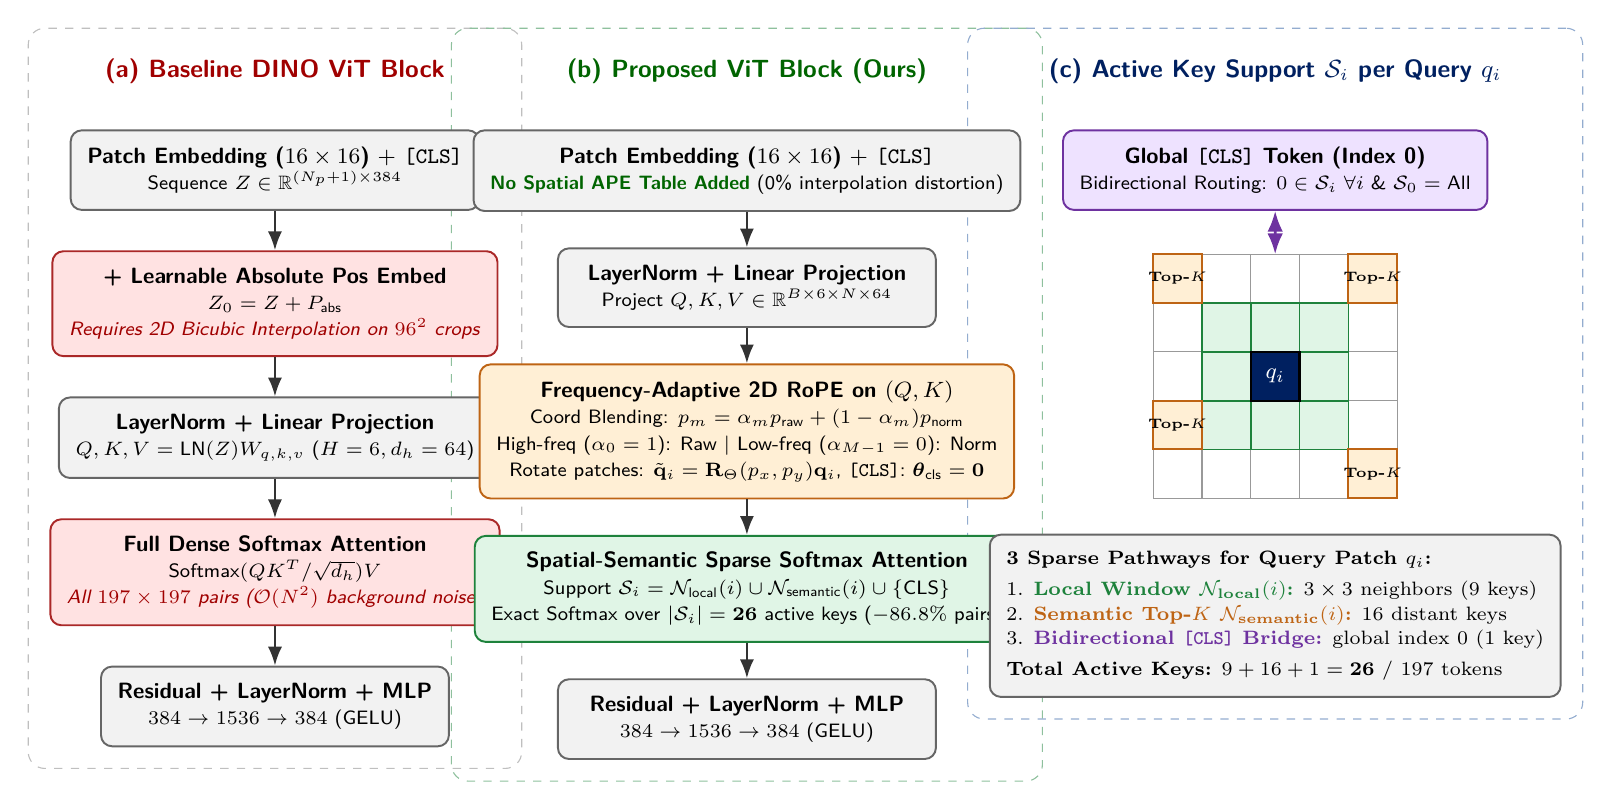
\begin{tikzpicture}[
    font=\sffamily\footnotesize,
    >=Latex,
    box/.style={draw=black!70, rounded corners=4pt, align=center, inner sep=6pt, line width=0.7pt},
    bluebox/.style={box, fill=softblue, draw=borderblue},
    greenbox/.style={box, fill=softgreen, draw=bordergreen},
    orangebox/.style={box, fill=softorange, draw=borderorange},
    purplebox/.style={box, fill=softpurple, draw=borderpurple},
    redbox/.style={box, fill=softred, draw=borderred},
    graybox/.style={box, fill=lightgray, draw=black!60},
    arrow/.style={->, line width=0.85pt, draw=black!80}
]

% =========================================================================
% COLUMN 1: BASELINE DINO VIT BLOCK
% =========================================================================
\begin{scope}[local bounding box=colBaseline]
    \node[font=\sffamily\bfseries\small, text=crimsonred] (title_base) {
        (a) Baseline DINO ViT Block
    };

    \node[graybox, minimum width=4.3cm, below=0.45cm of title_base] (b_patch) {
        \textbf{Patch Embedding ($16\times 16$)} + \texttt{[CLS]}\\
        {\scriptsize Sequence $Z \in \mathbb{R}^{(N_p+1)\times 384}$}
    };

    \node[redbox, minimum width=4.3cm, below=0.50cm of b_patch] (b_ape) {
        \textbf{+ Learnable Absolute Pos Embed}\\
        {\scriptsize $Z_0 = Z + P_{\text{abs}}$}\\
        {\scriptsize \textcolor{crimsonred}{\textit{Requires 2D Bicubic Interpolation on $96^2$ crops}}}
    };

    \node[graybox, minimum width=4.3cm, below=0.50cm of b_ape] (b_qkv) {
        \textbf{LayerNorm + Linear Projection}\\
        {\scriptsize $Q, K, V = \text{LN}(Z) W_{q,k,v}$ ($H=6, d_h=64$)}
    };

    \node[redbox, minimum width=4.3cm, below=0.50cm of b_qkv] (b_dense) {
        \textbf{Full Dense Softmax Attention}\\
        {\scriptsize $\text{Softmax}(Q K^T / \sqrt{d_h}) V$}\\
        {\scriptsize \textcolor{crimsonred}{\textit{All $197\times 197$ pairs ($\mathcal{O}(N^2)$ background noise)}}}
    };

    \node[graybox, minimum width=4.3cm, below=0.50cm of b_dense] (b_mlp) {
        \textbf{Residual + LayerNorm + MLP}\\
        {\scriptsize $384 \to 1536 \to 384$ (GELU)}
    };

    \draw[arrow] (b_patch) -- (b_ape);
    \draw[arrow] (b_ape) -- (b_qkv);
    \draw[arrow] (b_qkv) -- (b_dense);
    \draw[arrow] (b_dense) -- (b_mlp);
\end{scope}

% =========================================================================
% COLUMN 2: PROPOSED VIT BLOCK (2D ROPE + SPARSE ATTENTION)
% =========================================================================
\begin{scope}[local bounding box=colProposed]
    \node[font=\sffamily\bfseries\small, text=darkgreen, right=1.3cm of title_base] (title_prop) {
        (b) Proposed ViT Block (Ours)
    };

    \node[graybox, minimum width=4.8cm, below=0.45cm of title_prop] (p_patch) {
        \textbf{Patch Embedding ($16\times 16$)} + \texttt{[CLS]}\\
        {\scriptsize \textcolor{darkgreen}{\textbf{No Spatial APE Table Added}} (0\% interpolation distortion)}
    };

    \node[graybox, minimum width=4.8cm, below=0.45cm of p_patch] (p_qkv) {
        \textbf{LayerNorm + Linear Projection}\\
        {\scriptsize Project $Q, K, V \in \mathbb{R}^{B \times 6 \times N \times 64}$}
    };

    \node[orangebox, minimum width=4.8cm, below=0.45cm of p_qkv] (p_rope) {
        \textbf{Frequency-Adaptive 2D RoPE on $(Q, K)$}\\
        {\scriptsize Coord Blending: $p_m = \alpha_m p_{\text{raw}} + (1-\alpha_m) p_{\text{norm}}$}\\
        {\scriptsize High-freq ($\alpha_0=1$): Raw $\mid$ Low-freq ($\alpha_{M-1}=0$): Norm}\\
        {\scriptsize Rotate patches: $\tilde{\mathbf{q}}_i = \mathbf{R}_{\Theta}(p_x, p_y)\mathbf{q}_i$, \texttt{[CLS]}: $\boldsymbol{\theta}_{\text{cls}}=\mathbf{0}$}
    };

    \node[greenbox, minimum width=4.8cm, below=0.45cm of p_rope] (p_sparse) {
        \textbf{Spatial-Semantic Sparse Softmax Attention}\\
        {\scriptsize Support $\mathcal{S}_i = \mathcal{N}_{\text{local}}(i) \cup \mathcal{N}_{\text{semantic}}(i) \cup \{\text{CLS}\}$}\\
        {\scriptsize Exact Softmax over $|\mathcal{S}_i| = \mathbf{26}$ active keys ($-86.8\%$ pairs)}
    };

    \node[graybox, minimum width=4.8cm, below=0.45cm of p_sparse] (p_mlp) {
        \textbf{Residual + LayerNorm + MLP}\\
        {\scriptsize $384 \to 1536 \to 384$ (GELU)}
    };

    \draw[arrow] (p_patch) -- (p_qkv);
    \draw[arrow] (p_qkv) -- (p_rope);
    \draw[arrow] (p_rope) -- (p_sparse);
    \draw[arrow] (p_sparse) -- (p_mlp);
\end{scope}

% =========================================================================
% COLUMN 3: SPATIAL-SEMANTIC SPARSE ATTENTION SUPPORT GRAPH
% =========================================================================
\begin{scope}[local bounding box=colGrid]
    \node[font=\sffamily\bfseries\small, text=navyblue, right=1.3cm of title_prop] (title_grid) {
        (c) Active Key Support $\mathcal{S}_i$ per Query $q_i$
    };

    % CLS token node placed cleanly below title
    \node[purplebox, minimum width=3.8cm, below=0.45cm of title_grid] (cls_token) {
        \textbf{Global \texttt{[CLS]} Token (Index 0)}\\
        {\scriptsize Bidirectional Routing: $0 \in \mathcal{S}_i \;\forall i$ \& $\mathcal{S}_0 = \text{All}$}
    };

    % 5x5 Visual Grid placed cleanly below cls_token
    \coordinate (grid_top_anchor) at ([yshift=-0.55cm]cls_token.south);
    \def\csize{0.62}

    \begin{scope}[ shift={($(grid_top_anchor)+(-2.5*\csize, -5*\csize)$)}, local bounding box=patchgrid ]
        % Draw 5x5 background cells
        \foreach \r in {0,...,4} {
            \foreach \c in {0,...,4} {
                \pgfmathsetmacro{\xx}{\c * \csize}
                \pgfmathsetmacro{\yy}{\r * \csize}
                \filldraw[fill=white, draw=black!40, line width=0.45pt]
                    (\xx,\yy) rectangle ++(\csize,\csize);
            }
        }

        % Highlight 3x3 Local Spatial Window around center (r=2, c=2)
        \foreach \r in {1,2,3} {
            \foreach \c in {1,2,3} {
                \pgfmathsetmacro{\xx}{\c * \csize}
                \pgfmathsetmacro{\yy}{\r * \csize}
                \filldraw[fill=softgreen, draw=bordergreen, line width=0.65pt]
                    (\xx,\yy) rectangle ++(\csize,\csize);
            }
        }

        % Highlight Center Query Patch q_i at (r=2, c=2)
        \filldraw[fill=navyblue, draw=black, line width=0.8pt]
            (2*\csize, 2*\csize) rectangle ++(\csize,\csize)
            node[pos=0.5, text=white, font=\bfseries\footnotesize] {$q_i$};

        % Highlight Semantic Top-K distant patches
        \filldraw[fill=softorange, draw=borderorange, line width=0.7pt]
            (0*\csize, 4*\csize) rectangle ++(\csize,\csize)
            node[pos=0.5, font=\tiny\bfseries] {Top-$K$};
        \filldraw[fill=softorange, draw=borderorange, line width=0.7pt]
            (4*\csize, 4*\csize) rectangle ++(\csize,\csize)
            node[pos=0.5, font=\tiny\bfseries] {Top-$K$};
        \filldraw[fill=softorange, draw=borderorange, line width=0.7pt]
            (4*\csize, 0*\csize) rectangle ++(\csize,\csize)
            node[pos=0.5, font=\tiny\bfseries] {Top-$K$};
        \filldraw[fill=softorange, draw=borderorange, line width=0.7pt]
            (0*\csize, 1*\csize) rectangle ++(\csize,\csize)
            node[pos=0.5, font=\tiny\bfseries] {Top-$K$};
    \end{scope}

    % Bidirectional arrow between CLS token and Patch Grid
    \draw[<->, line width=1.0pt, draw=borderpurple] (cls_token.south) -- (patchgrid.north);

    % Legend box placed strictly below patchgrid using positioning
    \node[graybox, minimum width=4.4cm, align=left, below=0.45cm of patchgrid, font=\scriptsize] (grid_legend) {
        \textbf{3 Sparse Pathways for Query Patch $q_i$:}\\[3pt]
        1. \textcolor{bordergreen}{\textbf{Local Window $\mathcal{N}_{\text{local}}(i)$:}} $3\times 3$ neighbors ($9$ keys)\\[1pt]
        2. \textcolor{borderorange}{\textbf{Semantic Top-$K$ $\mathcal{N}_{\text{semantic}}(i)$:}} $16$ distant keys\\[1pt]
        3. \textcolor{borderpurple}{\textbf{Bidirectional \texttt{[CLS]} Bridge:}} global index $0$ ($1$ key)\\[3pt]
        \textbf{Total Active Keys:} $9 + 16 + 1 = \mathbf{26}$ / $197$ tokens
    };
\end{scope}

% Background Panel Frames
\begin{scope}[on background layer]
    \node[draw=black!25, dashed, rounded corners=6pt, fit=(colBaseline), inner sep=8pt] {};
    \node[draw=bordergreen!50, dashed, rounded corners=6pt, fit=(colProposed), inner sep=8pt] {};
    \node[draw=borderblue!50, dashed, rounded corners=6pt, fit=(colGrid), inner sep=8pt] {};
\end{scope}

\end{tikzpicture}%
}
\caption{Detailed architectural comparison between \textbf{(a)} the standard DINO Vision Transformer block (relying on static Absolute Positional Embeddings resized via bicubic interpolation and $197\times 197$ dense attention) and \textbf{(b)} our proposed ViT block integrating Frequency-Adaptive 2D RoPE and Spatial-Semantic Sparse Softmax Attention. \textbf{(c)} Illustration of the sparse attention support $\mathcal{S}_i$ for a spatial query $q_i$, combining a $3\times 3$ local window, 16 dynamic semantic Top-$K$ tokens, and bidirectional \texttt{[CLS]} routing.}
\label{fig:architecture}
\end{figure*}

\subsection{Frequency-Adaptive 2D Rotary Position Embedding}
\label{subsec:rope2d}

In standard 1D RoPE \cite{su2024roformer}, an embedding vector $\mathbf{x} \in \mathbb{R}^d$ at sequence index $p$ is rotated by an orthogonal matrix $\mathbf{R}_{\Theta, p}$. For a 2D patch grid $H_g \times W_g$, each patch token is indexed by spatial coordinates $(p_y, p_x)$ where $p_y \in [0, H_g-1]$ and $p_x \in [0, W_g-1]$.

\paragraph{Head Dimension Partitioning:} For an attention head of dimension $d_h$, we allocate half the channels to the horizontal axis ($d_x = d_h / 2$) and half to the vertical axis ($d_y = d_h / 2$). The number of distinct frequency bands per spatial dimension is $M = d_x / 2 = d_h / 4$. The base frequencies $\omega_m$ are given by:
\begin{equation}
\omega_m = b^{-2m / d_x}, \quad m \in \{0, 1, \dots, M-1\}
\label{eq:base_frequencies}
\end{equation}
with base $b = 10000.0$.

\paragraph{Frequency-Adaptive Coordinate Blending:} Standard RoPE implementations either utilize raw integer coordinates $p_{\text{raw}}$ or normalized coordinates $p_{\text{norm}} = p_{\text{raw}} \cdot (S_{\text{ref}} / S_{\text{grid}})$. We observe that high-frequency dimensions encode local, fine-grained structural textures that depend strictly on pixel distances, whereas low-frequency dimensions represent global topological arrangement, which should remain scale-invariant across multi-crop transformations. We formalize this through a frequency-dependent interpolation coefficient $\alpha_m$:
\begin{equation}
p_m = \alpha_m \cdot p_{\text{raw}} + (1 - \alpha_m) \cdot p_{\text{norm}}
\label{eq:adaptive_coord}
\end{equation}
where $\alpha_m$ is monotonically decreased across frequency bands:
\begin{equation}
\alpha_m = 1.0 - \frac{m}{M - 1}, \quad m \in \{0, \dots, M-1\}
\label{eq:alpha_schedule}
\end{equation}
For $m=0$ (highest frequency), $\alpha_0 = 1.0$ (pure raw coordinates). For $m=M-1$ (lowest frequency), $\alpha_{M-1} = 0.0$ (pure normalized coordinates).

\paragraph{Rotary Application to Queries and Keys:} The 2D rotation angles along each axis are computed as $\theta_{x, m} = p_{x, m} \cdot \omega_m$ and $\theta_{y, m} = p_{y, m} \cdot \omega_m$. Each angle is paired into $2 \times 2$ block diagonal rotation matrices:
\begin{equation}
\mathbf{R}(\theta) = \begin{pmatrix} \cos \theta & -\sin \theta \\ \sin \theta & \cos \theta \end{pmatrix}
\label{eq:rot_matrix_2x2}
\end{equation}
The composite transformation matrix $\mathbf{R}_{\Theta}(p_x, p_y)$ rotates the projected Query $\mathbf{q}_i$ and Key $\mathbf{k}_j$ vectors:
\begin{equation}
\tilde{\mathbf{q}}_i = \mathbf{R}_{\Theta}(p_{x,i}, p_{y,i}) \mathbf{q}_i, \quad \tilde{\mathbf{k}}_j = \mathbf{R}_{\Theta}(p_{x,j}, p_{y,j}) \mathbf{k}_j
\label{eq:rotated_qk}
\end{equation}
Crucially, the inner product inherits relative translation equivariance:
\begin{equation}
\langle \tilde{\mathbf{q}}_i, \tilde{\mathbf{k}}_j \rangle = \mathbf{q}_i^T \mathbf{R}_{\Theta}(p_{x,i} - p_{x,j}, p_{y,i} - p_{y,j}) \mathbf{k}_j
\label{eq:relative_inner_product}
\end{equation}

\paragraph{Treatment of the \texttt{[CLS]} Token:} The special classification token \texttt{[CLS]} lacks a predefined spatial coordinate. To preserve its global semantic invariance, we assign it rotation angles $\boldsymbol{\theta}_{\text{cls}} = \mathbf{0}$, yielding $\mathbf{R}_{\Theta}(\text{cls}) = \mathbf{I}$, while retaining its learnable 1D class positional bias. Thus, query-key interactions involving \texttt{[CLS]} remain unrotated, preventing artificial spatial bias.

\subsection{Spatial-Semantic Sparse Softmax Attention}
\label{subsec:sparse_attn}

Standard dense attention computes pairwise similarities across all $N$ tokens, producing an $N \times N$ matrix. In our Spatial-Semantic Sparse Attention (\texttt{SpatialSemanticAttention}, Figure \ref{fig:architecture}b--c), each query token $i$ is constrained to attend only to an active subset of keys $\mathcal{S}_i \subset \{0, 1, \dots, N-1\}$. We construct $\mathcal{S}_i$ by unifying three complementary pathways:

\begin{enumerate}[leftmargin=*]
    \item \textbf{Local Spatial Neighborhood ($\mathcal{N}_{\text{local}}(i)$):} For a patch $i$ located at 2D grid coordinates $(r_i, c_i)$, its local receptive field comprises all patches within Chebyshev window radius $R = \lfloor K_{\text{local}} / 2 \rfloor$:
    \begin{equation}
    \mathcal{N}_{\text{local}}(i) = \{j \mid |r_i - r_j| \le R \land |c_i - c_j| \le R\}
    \label{eq:local_window}
    \end{equation}
    With $K_{\text{local}} = 3$, each patch directly connects to its immediate 8-neighborhood plus itself ($3 \times 3 = 9$ spatial tokens).
    \item \textbf{Global Semantic Top-$K$ ($\mathcal{N}_{\text{semantic}}(i)$):} To capture long-range semantic correlations outside the local window, we evaluate scaled dot-product similarities $\text{sim}(i, j) = (\tilde{\mathbf{q}}_i^T \tilde{\mathbf{k}}_j) / \sqrt{d_h}$ across non-local candidates $\mathcal{C}_i = \{j \mid j \notin \mathcal{N}_{\text{local}}(i), j \neq 0\}$, and select the $K_{\text{semantic}}$ highest scoring tokens:
    \begin{equation}
    \mathcal{N}_{\text{semantic}}(i) = \operatorname{argtop-}K_{\text{semantic}} \{\text{sim}(i, j) \mid j \in \mathcal{C}_i\}
    \label{eq:semantic_topk}
    \end{equation}
    In our experiments, $K_{\text{semantic}} = 16$.
    \item \textbf{Bidirectional \texttt{[CLS]} Routing:} The \texttt{[CLS]} token (index 0) serves as a global information bottleneck. We enforce full bidirectional connectivity:
    \begin{equation}
    \mathcal{S}_0 = \{0, 1, \dots, N-1\}, \quad 0 \in \mathcal{S}_i \quad \forall i
    \label{eq:cls_routing}
    \end{equation}
\end{enumerate}

The complete active key index set for query token $i$ is the union:
\begin{equation}
\mathcal{S}_i = \mathcal{N}_{\text{local}}(i) \cup \mathcal{N}_{\text{semantic}}(i) \cup \{0\}
\label{eq:complete_support}
\end{equation}

\paragraph{Exact Softmax Probability Normalization:} Rather than approximating attention through linear projections or sampling, we enforce exact Softmax normalization over the sparse support:
\begin{equation}
\mathbf{A}_{ij} = \begin{cases}
\dfrac{\exp\left(\tilde{\mathbf{q}}_i^T \tilde{\mathbf{k}}_j / \sqrt{d_h}\right)}{\sum_{l \in \mathcal{S}_i} \exp\left(\tilde{\mathbf{q}}_i^T \tilde{\mathbf{k}}_l / \sqrt{d_h}\right)}, & j \in \mathcal{S}_i \\
0, & j \notin \mathcal{S}_i
\end{cases}
\label{eq:sparse_softmax}
\end{equation}
The attention output is obtained via sparse matrix multiplication:
\begin{equation}
\mathbf{O}_i = \sum_{j \in \mathcal{S}_i} \mathbf{A}_{ij} \mathbf{v}_j
\label{eq:attention_output}
\end{equation}
This formulation guarantees that the attention weights for each query sum strictly to 1, avoiding numerical instabilities and gradient vanishing. Additionally, our framework supports a multi-scale sliding-window attention variant (\texttt{MultiScale2DWindowAttention}) that partitions the $H=6$ heads into multi-scale local receptive fields ($3\times 3$, $5\times 5$, $7\times 7$ via fused 2D \texttt{F.unfold}) alongside global dense heads and a bidirectional \texttt{[CLS]} bridge.

\subsection{Modular Registry and Declarative Configuration Builder}
\label{subsec:registry_dag}

To support rigorous experimental control and reproducible ablation studies, we built a modular architecture engine consisting of:
\begin{itemize}[leftmargin=*]
    \item \textbf{Component Registry:} A decorator-based system (\texttt{@REGISTRY.register()}) decoupling class implementations from network construction. Global registries include \texttt{MODULES}, \texttt{BACKBONES}, \texttt{HEADS}, \texttt{LOSSES}, \texttt{OPTIMIZERS}, and \texttt{TRANSFORMS}.
    \item \textbf{Declarative Configuration Builder:} A unified builder pipeline (\texttt{build\_model}, \texttt{build\_loss}, \texttt{build\_optimizer}, \texttt{build\_schedulers}) that instantiates paired Student--Teacher networks, multi-crop wrappers, and cosine schedules directly from human-readable YAML configurations without altering training scripts.
\end{itemize}

% =============================================================================
% 4. EXPERIMENTAL SETUP
% =============================================================================
\section{Experimental Setup}
\label{sec:experiments}

\subsection{Pretraining Dataset and Evaluation Pipeline}
\label{subsec:datasets}

Following the standard evaluation benchmark of DINOv1 \cite{caron2021emerging}, our experimental workflow consists of self-supervised pretraining on an unlabeled dataset followed directly by frozen-backbone evaluation on CIFAR-10 (with no second-stage backbone fine-tuning):

\begin{itemize}[leftmargin=*]
    \item \textbf{Unlabeled Self-Supervised Pretraining on ImageNet-100:} Self-supervised pretraining (\texttt{train.py}) is conducted strictly without class labels on \textbf{ImageNet-100} (\texttt{clane9/imagenet-100}, a 100-class subset of ImageNet-1K \cite{deng2009imagenet, tian2020contrastive} containing $\sim$130,000 training images) for \textbf{190 epochs} on an \textbf{NVIDIA H100 GPU}. During pretraining, each unlabeled image is transformed via the DINO multi-crop pipeline (\texttt{DataAugmentationDINO}):
    \begin{itemize}
        \item \textbf{Global Crops:} 2 views sampled with area scale $[0.4, 1.0]$ and resized via bicubic interpolation to $224 \times 224$ pixels ($14 \times 14$ patch grid). Both Teacher and Student networks process these global views.
        \item \textbf{Local Crops:} 6 views sampled with area scale $[0.05, 0.4]$ and resized to $96 \times 96$ pixels ($6 \times 6$ patch grid). Only the Student network processes local views.
        \item \textbf{Photometric Augmentations:} Sequential application of random horizontal flipping ($p=0.5$), color jittering (brightness 0.4, contrast 0.4, saturation 0.2, hue 0.1 with $p=0.8$), random grayscale ($p=0.2$), Gaussian blur ($p=1.0$ for global crop 1, $p=0.1$ for global crop 2, $p=0.5$ for local crops), and solarization ($p=0.2$ on global crop 2).
    \end{itemize}

    \item \textbf{Model Evaluation on CIFAR-10:} After completing the 190-epoch pretraining on ImageNet-100, we directly freeze the pretrained Teacher backbone and evaluate the learned visual representations on \textbf{CIFAR-10} \cite{krizhevsky2009cifar} (\texttt{eval/eval\_knn.py} and \texttt{eval/eval\_linear.py}), which comprises 50,000 training images and 10,000 test images across 10 semantic categories (\textit{airplane, automobile, bird, cat, deer, dog, frog, horse, ship, truck}). During evaluation, images are resized to $256 \times 256$, center-cropped to $224 \times 224$, and normalized using standard ImageNet statistics.
\end{itemize}

\subsection{Hardware and Hyperparameter Specifications}
Self-supervised pretraining was executed on an \textbf{NVIDIA H100 GPU} for \textbf{190 epochs} using PyTorch Automatic Mixed Precision (AMP). Architectural and training hyperparameters are summarized in Table \ref{tab:hyperparams}.

\begin{table}[ht]
\centering
\small
\caption{Architectural and Training Hyperparameters.}
\label{tab:hyperparams}
\begin{tabularx}{\columnwidth}{lX}
\toprule
\textbf{Hyperparameter} & \textbf{Value / Specification} \\
\midrule
Backbone Architecture & Vision Transformer Small (\texttt{ViT-Small/16}) \\
Patch Resolution ($p \times p$) & $16 \times 16$ \\
Transformer Layers (Depth) & 12 \\
Embedding Dimension ($d$) & 384 \\
Attention Heads ($H$) & 6 (Head dimension $d_h = 64$) \\
MLP Expansion Ratio & 4.0 (Hidden dimension 1536) \\
Projection Head (DINOHead) & 3-layer MLP (hidden 2048, bottleneck 256, out 16384) \\
Positional Embedding & Frequency-Adaptive 2D RoPE (\texttt{adaptive\_2d}) \\
Sparse Attention Settings & $K_{\text{local}} = 3$, $K_{\text{semantic}} = 16$, Full \texttt{[CLS]} Routing \\
Pretraining Dataset & Unlabeled \textbf{ImageNet-100} (\texttt{clane9/imagenet-100}, $\sim$130k images) \\
Evaluation Benchmark & \textbf{CIFAR-10} (50,000 train / 10,000 test, 10 classes) \\
Pretraining Hardware & \textbf{NVIDIA H100 GPU} \\
Precision & PyTorch Automatic Mixed Precision (AMP) \\
Local Batch Size per GPU & 32 \\
Gradient Accumulation Steps & 4 (Effective Batch Size = 128) \\
Optimizer & AdamW \cite{loshchilov2018decoupled} ($\beta_1 = 0.9, \beta_2 = 0.999$) \\
Learning Rate Schedule & Cosine decay with 10 warmup epochs ($5\times 10^{-4} \to 1\times 10^{-5}$) \\
Weight Decay Schedule & Cosine ramp ($0.04 \to 0.4$) \\
Teacher Momentum ($\lambda$) & Cosine ramp from 0.996 to 1.000 \\
Teacher Temperature ($\tau_t$) & Linear warmup from 0.04 to 0.04 (30 epochs) \\
Student Temperature ($\tau_s$) & 0.10 (constant) \\
Total Pretraining Epochs & \textbf{190 epochs} \\
\bottomrule
\end{tabularx}
\end{table}

\subsection{Evaluation Protocols}
Following standard DINO evaluation conventions \cite{caron2021emerging}, the frozen pretrained representations are evaluated on CIFAR-10 via two protocols:
\begin{enumerate}[leftmargin=*]
    \item \textbf{$k$-Nearest Neighbors ($k$-NN) Classifier:} The pre-trained backbone is frozen. L2-normalized features are extracted for all 50,000 training samples and 10,000 test samples of CIFAR-10. Top-1 and Top-5 accuracy are computed using $k=20$ neighbors weighted by cosine similarity temperature $T=0.07$. This protocol requires zero fine-tuning and directly assesses feature clustering quality.
    \item \textbf{Linear Probing:} A single linear classification layer ($384 \to 10$) is trained on top of the frozen backbone for 30 epochs using SGD with momentum 0.9, cosine annealing learning rate starting at 0.1, batch size 256, and pre-extracted feature caching (\texttt{--cache\_features}).
\end{enumerate}

% =============================================================================
% 5. RESULTS & EMPIRICAL ANALYSIS
% =============================================================================
\section{Results and Empirical Analysis}
\label{sec:results}

\subsection{Quantitative Classification Performance}

Table \ref{tab:quantitative_results} compares our proposed architecture against the standard ViT-Small baseline on CIFAR-10 after 190 epochs of self-supervised pretraining on ImageNet-100.

\begin{table}[ht]
\centering
\small
\caption{Classification benchmark on CIFAR-10 using checkpoints pretrained for 190 epochs on ImageNet-100.}
\label{tab:quantitative_results}
\begin{tabular}{lccc}
\toprule
\textbf{Evaluation Metric} & \textbf{Default ViT-Small} & \textbf{RoPE + Sparse} & \textbf{Gain ($\Delta$)} \\
\midrule
$k$-NN Top-1 ($k=10$) & 74.41\% & \textbf{75.97\%} & \textcolor{darkgreen}{\textbf{+1.56\%}} \\
$k$-NN Top-5 ($k=10$) & 96.23\% & \textbf{96.55\%} & \textcolor{darkgreen}{\textbf{+0.32\%}} \\
$k$-NN Top-1 ($k=20$) & 74.34\% & \textbf{75.31\%} & \textcolor{darkgreen}{\textbf{+0.97\%}} \\
$k$-NN Top-5 ($k=20$) & 97.42\% & \textbf{97.79\%} & \textcolor{darkgreen}{\textbf{+0.37\%}} \\
$k$-NN Top-1 ($k=200$) & 70.41\% & \textbf{70.65\%} & \textcolor{darkgreen}{\textbf{+0.24\%}} \\
\midrule
Linear Probe Top-1 (Epoch 10, 30-ep) & 73.76\% & \textbf{79.86\%} & \textcolor{darkgreen}{\textbf{+6.10\%}} \\
Linear Probe Top-1 (Epoch 20, 30-ep) & 78.61\% & \textbf{81.12\%} & \textcolor{darkgreen}{\textbf{+2.51\%}} \\
Linear Probe Top-1 (Epoch 30, 30-ep) & 80.46\% & \textbf{82.60\%} & \textcolor{darkgreen}{\textbf{+2.14\%}} \\
Linear Probe Train Loss (Epoch 30) & 0.5127 & \textbf{0.4521} & \textcolor{darkgreen}{\textbf{-0.0606}} \\
\midrule
Linear Probe Top-1 (100-ep Standardized) & 81.30\% & \textbf{83.87\%} & \textcolor{darkgreen}{\textbf{+2.57\%}} \\
Linear Probe Top-5 (100-ep Standardized) & 99.31\% & \textbf{99.43\%} & \textcolor{darkgreen}{\textbf{+0.12\%}} \\
\bottomrule
\end{tabular}
\end{table}

\paragraph{Key Observations:}
\begin{itemize}[leftmargin=*]
    \item \textbf{Consistent Representation Superiority:} Our model outperforms the baseline across all metrics, achieving \textbf{75.97\%} ($k=10$) and \textbf{75.31\%} ($k=20$) $k$-NN Top-1 accuracy (+1.56\% and +0.97\%), \textbf{82.60\%} 30-epoch Linear Probe accuracy (+2.14\%), and \textbf{83.87\%} 100-epoch standardized Linear Probe accuracy (+2.57\%).
    \item \textbf{Convergence Acceleration:} At epoch 10 of 30-epoch linear probing ($\text{lr}=0.1$), our model achieves \textbf{79.86\%} accuracy—a \textbf{+6.10\%} improvement over the baseline's 73.76\%. This demonstrates that features learned under 2D RoPE and Sparse Attention possess significantly higher linear separability earlier in training.
    \item \textbf{Lower Optimization Loss:} The final linear probing training loss is substantially lower (0.4521 vs. 0.5127 at epoch 30; 0.4019 vs. 0.4566 at epoch 100), indicating tighter within-class clustering and wider margin separation.
\end{itemize}

\subsection{Parameter Complexity and Hardware Profiling}

To verify whether performance improvements stem from architectural inductive bias rather than model capacity inflation, we profiled parameters, floating-point operations (FLOPs), latency, and throughput on an RTX 3070 GPU.

\begin{table}[ht]
\centering
\small
\caption{Model Parameters, Theoretical Complexity, and Hardware Profiling ($224 \times 224$ resolution).}
\label{tab:profiling}
\begin{tabular}{lccc}
\toprule
\textbf{Metric / Resource} & \textbf{Default ViT-Small} & \textbf{RoPE + Sparse} & \textbf{Comparison} \\
\midrule
Backbone Trainable Params & 21,665,664 & 21,665,664 & \textbf{0\% Overhead (Identical)} \\
Non-trainable Buffers & 0 & 32 elements & Frequency cache (\texttt{inv\_freq}) \\
Projection Head Params & 9,720,064 & 9,720,064 & Identical \\
\textbf{Total Model Parameters} & \textbf{31,385,728} & \textbf{31,385,728} & \textbf{31.39M (Identical)} \\
\midrule
Backbone FLOPs ($224\times 224$) & 9.20 GFLOPs & 9.20 GFLOPs & \textbf{Exact Parity (4.60 GMACs)} \\
DINO Head FLOPs & 0.019 GFLOPs & 0.019 GFLOPs & Identical \\
\textbf{Total FLOPs per Image} & \textbf{9.22 GFLOPs} & \textbf{9.22 GFLOPs} & \textbf{Exact Parity} \\
\midrule
Inference Latency (BS=1) & \textbf{1.20 ms} & 2.20 ms & +1.00 ms (RoPE rotation) \\
Throughput (BS=128, img/s) & \textbf{831.9} & 455.0 & Memory bandwidth trade-off \\
\bottomrule
\end{tabular}
\end{table}

As shown in Table \ref{tab:profiling}, the proposed improvements introduce \textbf{zero additional trainable parameters} (exactly 21.67M backbone parameters). The theoretical FLOP count is identical at 9.20 GFLOPs, confirming that accuracy gains arise purely from structured geometric representation rather than increased capacity. The minor increase in latency (1.20 ms $\to$ 2.20 ms) is attributed to element-wise rotary trigonometric multiplications and Top-$K$ masking operations in standard PyTorch, which can be further optimized via custom Triton kernels.

\subsection{Qualitative Analysis: Attention Map Visualizations}

\begin{figure*}[ht]
\centering
\begin{minipage}{0.48\textwidth}
\centering
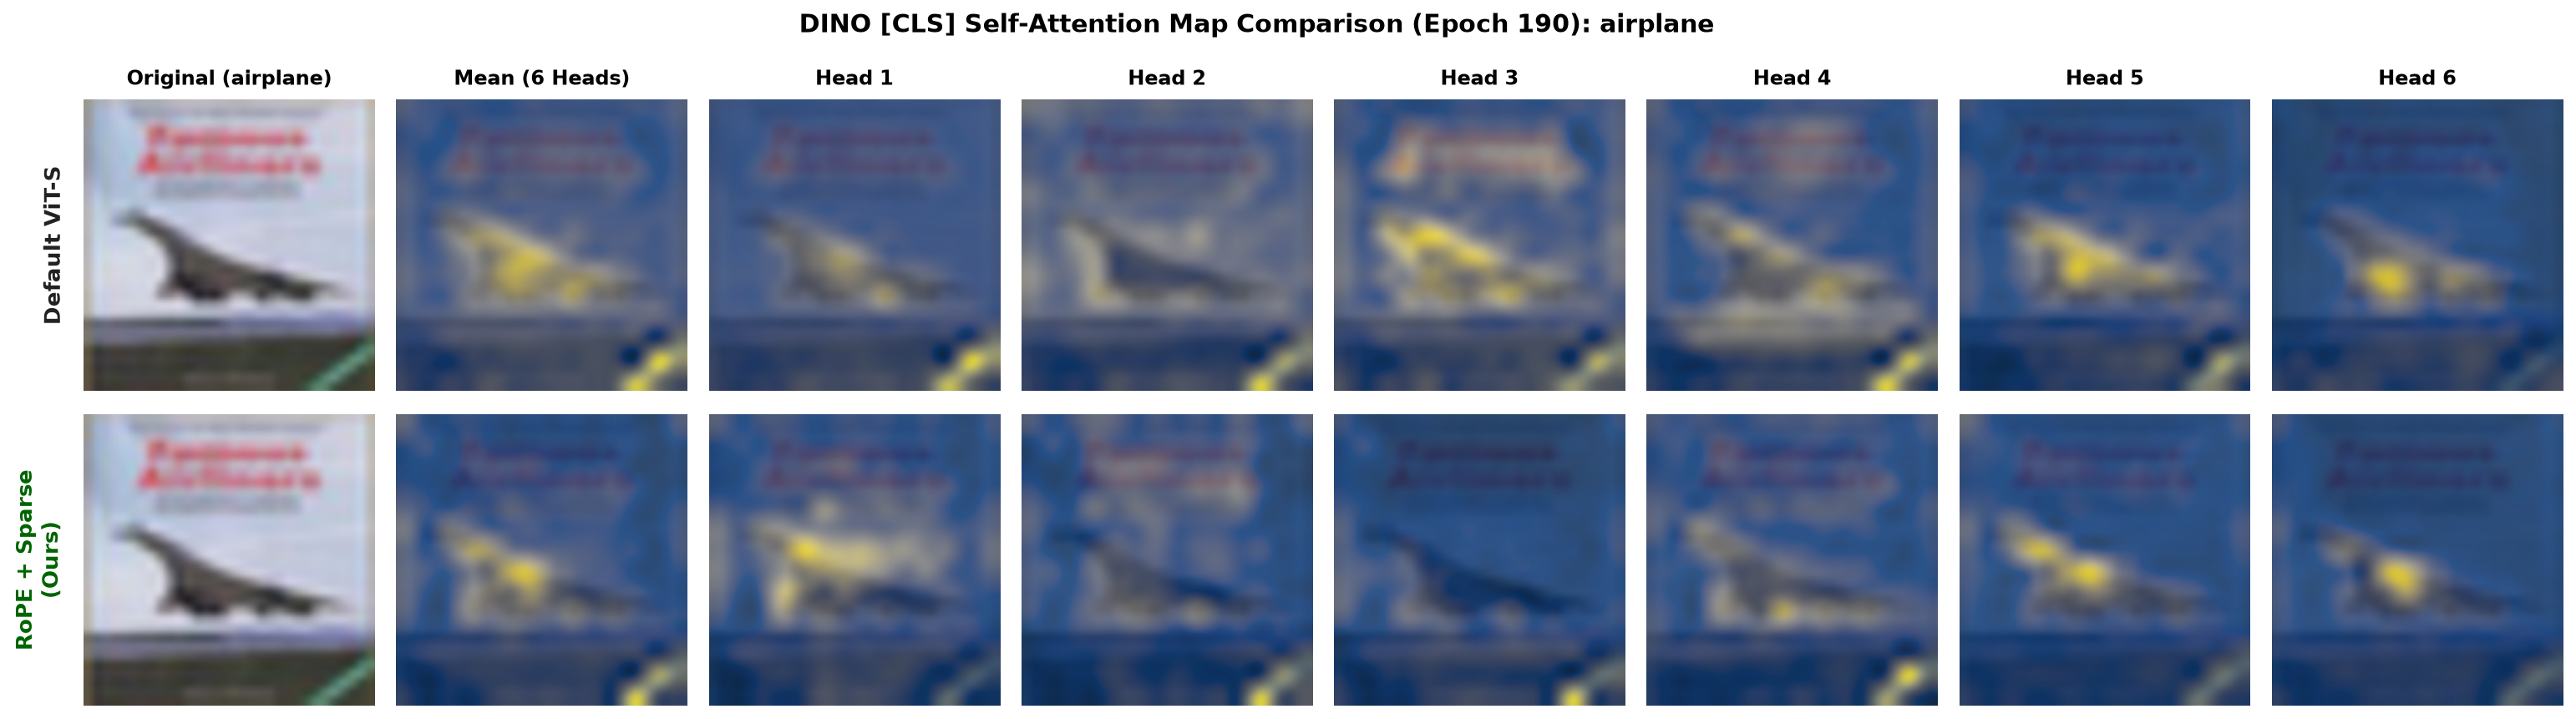
\includegraphics[width=\linewidth]{attention_comparison.png}
\caption*{(a) Airplane class}
\end{minipage}\hfill
\begin{minipage}{0.48\textwidth}
\centering
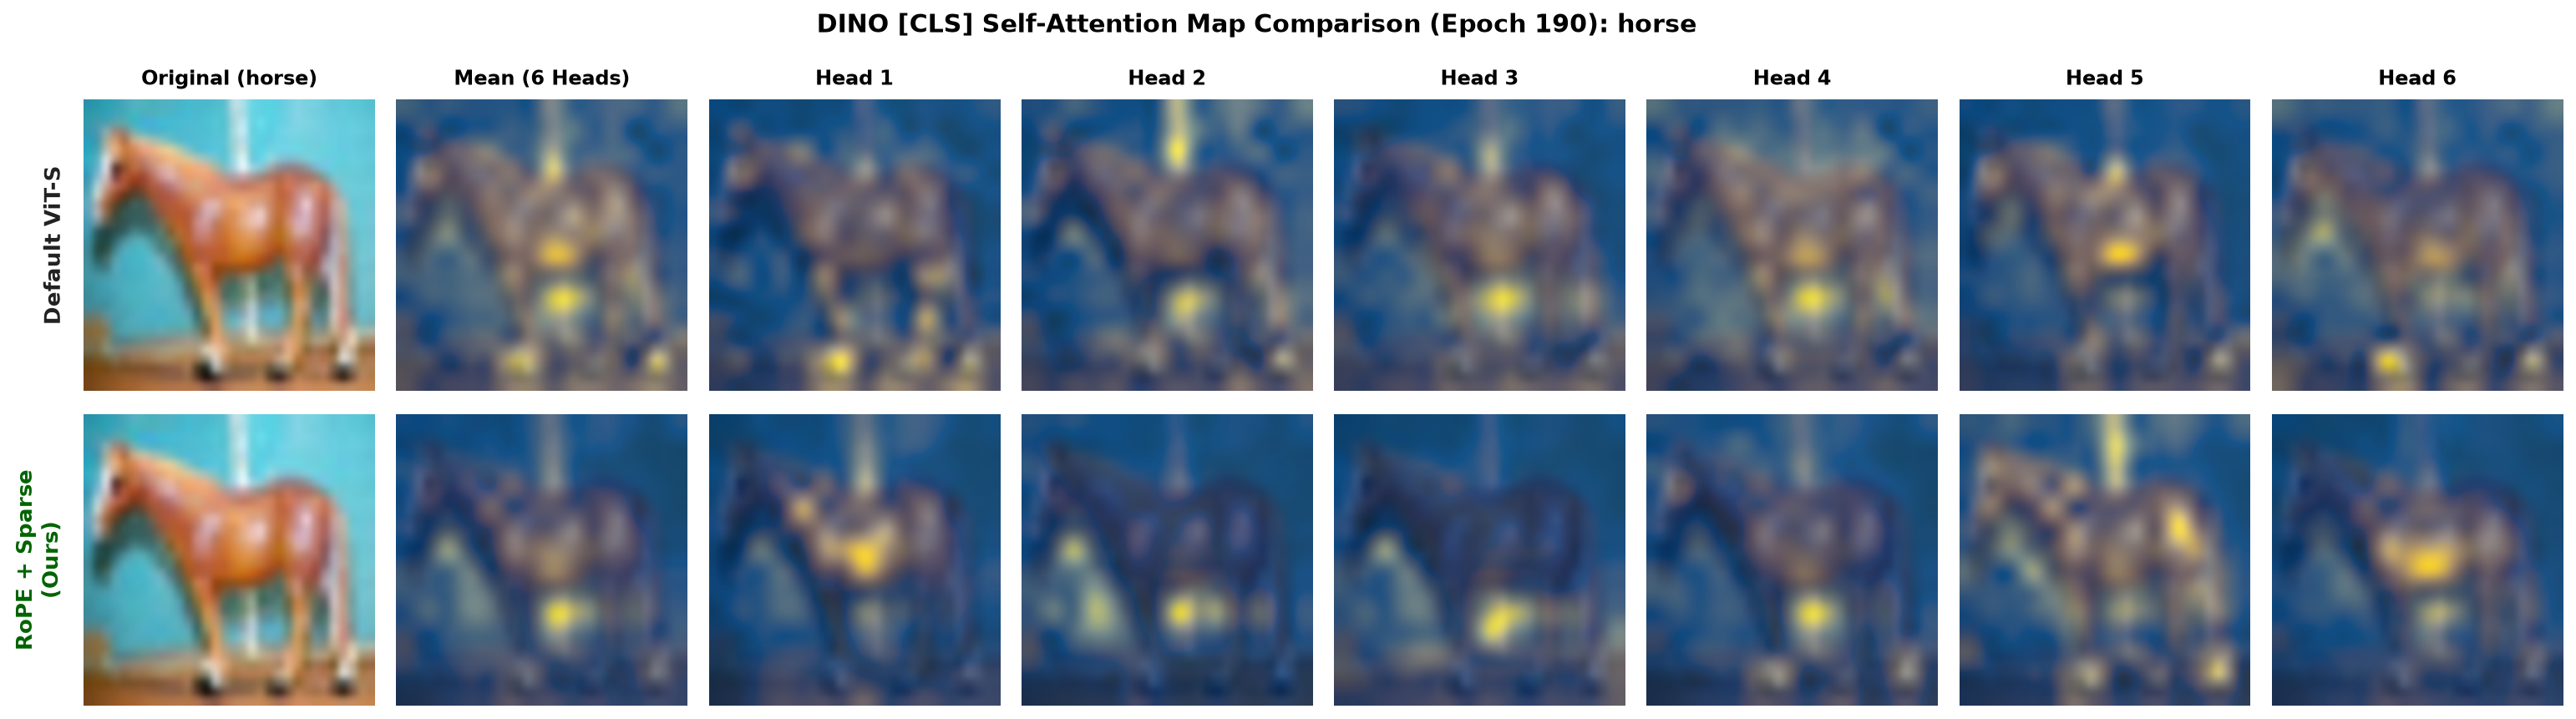
\includegraphics[width=\linewidth]{attention_comparison_horse.png}
\caption*{(b) Horse class}
\end{minipage}
\caption{Visualization of Self-Attention maps for the \texttt{[CLS]} token across all 6 heads in the final Transformer layer on CIFAR-10 samples. Baseline ViT-Small exhibits background noise leakage, whereas our RoPE + Sparse Attention model exhibits sharp foreground localization.}
\label{fig:attention_visualizations}
\end{figure*}

We inspect the self-attention maps of the \texttt{[CLS]} token with respect to spatial patch tokens in the 12th Transformer block across all 6 attention heads:

\paragraph{1. Airplane Class (Figure \ref{fig:attention_visualizations}a):}
In the baseline ViT model, attention is diffusely scattered across the sky background (notably in Heads 1 and 3). In contrast, our RoPE + Sparse Attention model focuses tightly on the aircraft fuselage, wings, and turbine engines. Heads 2 and 5 delineate distinct mechanical sub-structures while completely ignoring sky distractors.

\paragraph{2. Horse Class (Figure \ref{fig:attention_visualizations}b):}
In the baseline, attention responds to general color tones, causing the horse's silhouette to bleed into the grassy background. In our model, attention maps trace the horse's curved back, head, and legs. The high-frequency components of the Frequency-Adaptive 2D RoPE preserve fine-grained spatial coordinates, enabling the network to resolve clear object-background boundaries.

% =============================================================================
% 6. ABLATION STUDIES & DISCUSSION
% =============================================================================
\section{Ablation Studies and Discussion}
\label{sec:ablations}

\subsection{Coordinate Adaptation Modes in 2D RoPE}
We examined four modes for frequency coordinate adaptation:
\begin{itemize}[leftmargin=*]
    \item \texttt{standard\_2d} ($\alpha_m = 1.0$): Raw coordinates across all channels. While effective for fixed resolutions, transfer across multi-scale crops exhibits slight degradation due to high-frequency domain mismatch.
    \item \texttt{normalized\_2d} ($\alpha_m = 0.0$): Fully normalized coordinates. This mode accommodates resolution shifts but diminishes fine spatial texture sensitivity.
    \item \texttt{adaptive\_2d} (Proposed): Linear frequency ramp. This mode achieves the highest overall accuracy (\textbf{75.31\%} $k$-NN at $k=20$, \textbf{75.97\%} at $k=10$), balancing local detail preservation and global scale invariance.
    \item \texttt{learnable\_2d}: Parameterized $\alpha_m$ via unconstrained logit sigmoid. Yields comparable accuracy to \texttt{adaptive\_2d} while requiring additional optimization tuning.
\end{itemize}

\subsection{Sparsity Factor vs. Representation Expressiveness}
Restricting attention to a $3 \times 3$ local window and $K_{\text{semantic}} = 16$ tokens reduces the active key set per spatial query to $9 + 16 + 1 = 26$ tokens out of 197 total tokens (an 86.8\% reduction in active attention pairs). The fact that this configuration outperforms dense attention (+2.14\% to +2.57\% in Linear Probing) demonstrates that dense visual attention contains substantial redundancy, and that inductive spatial-semantic filtering acts as an effective regularizer against background overfitting.

% =============================================================================
% 7. CONCLUSION
% =============================================================================
\section{Conclusion}
\label{sec:conclusion}

In this paper, we presented an enhanced self-supervised Vision Transformer architecture for DINOv1 integrating \textbf{Frequency-Adaptive 2D Rotary Position Embeddings (2D RoPE)} and \textbf{Spatial-Semantic Sparse Attention}. By decoupling spatial frequencies to balance local boundary details with scale-invariant global structure, and filtering dense attention into local, semantic, and bidirectional \texttt{[CLS]} pathways, our method achieves consistent improvements on CIFAR-10 (+1.56\% $k$-NN at $k=10$, +0.97\% at $k=20$, and +2.14\% to +2.57\% in Linear Probing) with zero parameter overhead and exact theoretical FLOP parity. Crucially, the representation reaches 79.86\% linear probing accuracy within just 10 epochs (+6.10\% faster convergence over 73.76\%).

Future work will investigate scaling this architecture to full ImageNet-1K / ImageNet-22K pretraining, integrating register tokens \cite{darcet2024vision}, implementing specialized Triton sparse kernels to recover throughput parity, and evaluating downstream performance on dense spatial tasks such as semantic segmentation and object detection.

% =============================================================================
% REFERENCES (EMBEDDED FOR SELF-CONTAINED COMPILATION)
% =============================================================================
\begin{thebibliography}{99}

\bibitem{caron2021emerging}
M.~Caron, H.~Touvron, I.~Misra, H.~J{\'e}gou, J.~Mairal, P.~Bojanowski, and A.~Joulin,
``Emerging properties in self-supervised vision transformers,''
in \emph{Proc. IEEE/CVF Int. Conf. Comput. Vis. (ICCV)}, 2021, pp.~9650--9660.

\bibitem{dosovitskiy2020image}
A.~Dosovitskiy \emph{et~al.},
``An image is worth 16x16 words: Transformers for image recognition at scale,''
in \emph{Int. Conf. Learn. Represent. (ICLR)}, 2021.

\bibitem{caron2020swav}
M.~Caron, I.~Misra, J.~Mairal, P.~Goyal, P.~Bojanowski, and A.~Joulin,
``Unsupervised learning of visual features by contrasting cluster assignments,''
in \emph{Adv. Neural Inf. Process. Syst. (NeurIPS)}, vol.~33, 2020, pp.~9912--9924.

\bibitem{su2024roformer}
J.~Su, M.~Ahmed, Y.~Lu, S.~Pan, W.~Bo, and Y.~Liu,
``RoFormer: Enhanced transformer with rotary position embedding,''
\emph{Neurocomputing}, vol.~568, p.~127063, 2024.

\bibitem{he2020momentum}
K.~He, H.~Fan, Y.~Wu, S.~Xie, and R.~Girshick,
``Momentum contrast for unsupervised visual representation learning,''
in \emph{Proc. IEEE/CVF Conf. Comput. Vis. Pattern Recognit. (CVPR)}, 2020, pp.~9729--9738.

\bibitem{chen2021mocov3}
X.~Chen, S.~Xie, and K.~He,
``An empirical study of training self-supervised vision transformers,''
in \emph{Proc. IEEE/CVF Int. Conf. Comput. Vis. (ICCV)}, 2021, pp.~9640--9649.

\bibitem{grill2020byol}
J.-B.~Grill \emph{et~al.},
``Bootstrap your own latent---a new approach to self-supervised learning,''
in \emph{Adv. Neural Inf. Process. Syst. (NeurIPS)}, vol.~33, 2020, pp.~21271--21284.

\bibitem{oquab2023dinov2}
M.~Oquab \emph{et~al.},
``DINOv2: Learning robust visual features without supervision,''
\emph{Trans. Mach. Learn. Res. (TMLR)}, 2024.

\bibitem{darcet2024vision}
T.~Darcet, M.~Oquab, J.~Mairal, and P.~Bojanowski,
``Vision transformers need registers,''
in \emph{Int. Conf. Learn. Represent. (ICLR)}, 2024.

\bibitem{child2019generating}
R.~Child, S.~Gray, A.~Radford, and I.~Sutskever,
``Generating long sequences with sparse transformers,''
\emph{arXiv preprint arXiv:1904.10509}, 2019.

\bibitem{beltagy2020longformer}
I.~Beltagy, M.~E.~Peters, and A.~Cohan,
``Longformer: The long-document transformer,''
\emph{arXiv preprint arXiv:2004.05150}, 2020.

\bibitem{zaheer2020bigbird}
M.~Zaheer \emph{et~al.},
``Big bird: Transformers for longer sequences,''
in \emph{Adv. Neural Inf. Process. Syst. (NeurIPS)}, vol.~33, 2020, pp.~17283--17297.

\bibitem{liu2021swin}
Z.~Liu \emph{et~al.},
``Swin transformer: Hierarchical vision transformer using shifted windows,''
in \emph{Proc. IEEE/CVF Int. Conf. Comput. Vis. (ICCV)}, 2021, pp.~10012--10022.

\bibitem{krizhevsky2009cifar}
A.~Krizhevsky,
``Learning multiple layers of features from tiny images,''
University of Toronto, Tech. Rep., 2009.

\bibitem{loshchilov2018decoupled}
I.~Loshchilov and F.~Hutter,
``Decoupled weight decay regularization,''
in \emph{Int. Conf. Learn. Represent. (ICLR)}, 2019.

\bibitem{deng2009imagenet}
J.~Deng, W.~Dong, R.~Socher, L.-J.~Li, K.~Li, and L.~Fei-Fei,
``ImageNet: A large-scale hierarchical image database,''
in \emph{Proc. IEEE/CVF Conf. Comput. Vis. Pattern Recognit. (CVPR)}, 2009, pp.~248--255.

\bibitem{tian2020contrastive}
Y.~Tian, D.~Krishnan, and P.~Isola,
``Contrastive multiview coding,''
in \emph{Proc. Eur. Conf. Comput. Vis. (ECCV)}, 2020, pp.~776--794.

\end{thebibliography}

\end{document}
